\documentclass[11pt, oneside]{article}
\usepackage[utf8]{inputenc}                        % utf8
\usepackage[T1]{fontenc}                           % fix font encoding
\usepackage[english]{babel}                        % language
\usepackage{titling, geometry, hyperref, fancyhdr, algorithm}
\usepackage{amsmath, amssymb, amsthm}              % ams mathematical packages
\usepackage{physics, mathtools, bm}                % extra math packages
\usepackage{graphicx, subcaption, wrapfig}         % images
\usepackage{fvextra, textcomp, CJKutf8}            % misc. text formatting
\usepackage[autostyle, english=american]{csquotes} % quotes
\usepackage[shortlabels]{enumitem}                 % lists
\usepackage{tikz, pgfplots, tikz-network}          % plots and graphs
\usepackage[noend]{algpseudocode}                  % algorithm psuedocode
\usepackage[cache=true]{minted}                    % source code
\usepackage[style=ieee]{biblatex}                  % bibliography
\geometry{a4paper}

\pgfplotsset{compat=1.17}                          % version of pgfplots

\hypersetup{
  colorlinks=true,
  urlcolor=cyan,
  linkcolor=magenta
}

\setminted[]{
  linenos=false,
  breaklines=true,
  encoding=utf8,
  fontsize=\normalsize,
  frame=lines,
  framesep=2mm
}

% https://tex.stackexchange.com/questions/343494/minted-red-box-around-greek-characters
\makeatletter
\AtBeginEnvironment{minted}{\dontdofcolorbox}
\def\dontdofcolorbox{\renewcommand\fcolorbox[4][]{##4}}
\makeatother

\graphicspath{{./images/}}
\addbibresource{ref.bib}

\title{Missile Guidance in the Presence of Constant Error}
\author{Stephen Huan, in collaboration with
\href{https://github.com/GLaDOS-42}{Sergey Blinov}}
\date{September 28, 2021}

\begin{document}
\maketitle
% {\hypersetup{linkcolor=black}
% \tableofcontents
% }

\section{Problem Statement}

A missile is heading towards the origin at a constant speed, however, its
guidance system has an error --- it is always deflected by an angle of
\( \alpha \). How long will it take to reach the origin, compared to the
straight-line path? See \autoref{fig:missile} for a visual depiction.

\begin{figure}[h!]
  \centering
  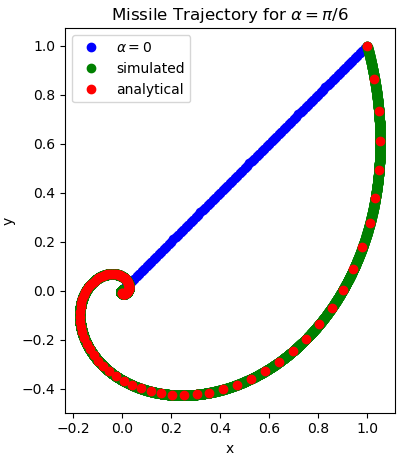
\includegraphics[scale=0.95]{missile.png}
  \caption{Missile path for \( \alpha = \frac{\pi}{6} \)}
  \label{fig:missile}
\end{figure}

\section{Solution}

Let \( \vec{r} \) be a vector representing the current position of the
missile. Normally we would move in the direction of \( -\vec{r} \), or the
vector pointing towards the origin. However, we're shifted by the angle of \(
\alpha \), so we multiply \( -\vec{r} \) by the rotation matrix \( T \):
\[ T(\alpha) = \begin{bmatrix} \cos \alpha & -\sin \alpha \\ 
                               \sin \alpha &  \sin \alpha 
                 \end{bmatrix} \]
\( T \) can be derived through standard linear algebra,
see \autoref{subsec:rotation} of the appendix.

\subsection{Differential Equation Setup}

So if our current position is \( \vec{r}_n \) at index \( n \), we have the
following recurrence for the next position over an infinitesimal step size:
\begin{align*}
  \tag{1} \label{eq:discrete}
  \vec{r}_{n + 1} &= \vec{r}_n + T(\alpha) (-\frac{\vec{r}_n}{\norm{\vec{r}_n}}) \Delta s
  \shortintertext{where we normalize the direction by dividing by its
    magnitude, and step \( \Delta s \), the amount we move the direction.
    Since we assume the direction doesn't change over our small enough
    step, then \( \Delta s \) is exactly the distance we move along the
    curve, or the arc length of the curve. Subtracting \( \vec{r}_n \)
    from both sides and dividing by \( \Delta s \),}
  \frac{\vec{r}_{n + 1} - \vec{r}_n}{\Delta s} &= T(\alpha) (-\frac{\vec{r}_n}{\norm{\vec{r}_n}}) 
  \shortintertext{In the limit as \( \Delta s \) tends towards 0,
    then this becomes a differential equation:}
  \tag{2} \label{eq:diffeq_arc}
  \frac{d \vec{r}}{ds} &= -T(\alpha) (\frac{\vec{r}}{\norm{\vec{r}}})
\end{align*}

However, equation \eqref{eq:diffeq_arc}, the differential equation
parameterized in terms of arc length, is difficult to solve, since
we're dividing by a highly nonlinear term. Instead, it would be nice
if the equation looked something like this, without the magnitude term:
\begin{align*}
  \tag{3} \label{eq:diffeq_time}
  \frac{d \vec{r}}{dt} = -T(\alpha) \vec{r}
\end{align*}

Luckily, I've hinted how we can use equation \eqref{eq:diffeq_time} without \(
\norm{\vec{r}} \): it simply represents a different \textit{parameterization}
of the same underlying curve, in particular in \enquote{time} rather than in
arc length. We know the arc length is the sum of changes over time:
\begin{align*}
  s(t) &= \int^t_0 \norm{\vec{r}'(\tau)} \, d\tau
  \shortintertext{so by taking the derivative, we recover the integrand:}
  \frac{ds}{dt} &= \norm{\vec{r}'(t)}
  \shortintertext{We know the what the derivative of
  \( \vec{r} \) is from differential equation \eqref{eq:diffeq_time},}
                &= \norm{-T(\alpha) \vec{r}}
  \shortintertext{Because a rotation doesn't change
    the magnitude of the vector, this is simply}
                &= \norm{\vec{r}}
  \shortintertext{So if we interpret \( \vec{r}(t) \)
    as a different parameterization, namely,
   \( \vec{r}(\int^t_0 \norm{\vec{r}'(\tau)} \, d\tau) \), then}
  \frac{d \vec{r}}{dt} &= \frac{d \vec{r}}{ds} \frac{ds}{dt} \\ 
  \shortintertext{Expanding \( \frac{d \vec{r}}{ds} \)
    from differential equation \eqref{eq:diffeq_arc},}
                       &= -T(\alpha) (\frac{\vec{r}(s)}{\norm{\vec{r}(s)}}) \norm{\vec{r}(s(t))} \\
                       &= -T(\alpha) \vec{r}(s(t)) \\
                       &= -T(\alpha) \vec{r}(t)
\end{align*}
The interesting thing is that the differential equation does not care which
parameter we access \( \vec{r} \) from, but only its \emph{actual position}.
Obviously \( \vec{r}(s) \) and \( \vec{r}(t) \) are equivalent if they give
the same vector \( \vec{r} \), as \( \vec{r}(s(t)) \) is parameterized in \(
t \) but through the intermediate \( s \).

From this exercise we realize that the differential equation
\eqref{eq:diffeq_time} without \( \norm{\vec{r}} \) is just a different
\emph{parameterization} of the same curve, where \( t \) varies from 0 to \(
\infty \), as the derivative \( \frac{d \vec{r}}{dt} \) becomes progressively
smaller, contributing less and less to the arc length.

In general, suppose we have an arbitrary parameterization \(
\vec{r}(f(t)) \) where \( f \) must fulfill certain properties:
it must be monotonically increasing so that increasing \( t \)
goes in the same direction as the original curve, and so that \(
f \) is bijective, i.e. we transition continuously and without
overlap, so \( f'(t) > 0 \). In that case, by chain rule,
\begin{align*}
  \frac{d \vec{r}(f(t))}{dt} &= f'(t) \vec{r}'(f(t))
  \shortintertext{Expanding from the
    differential equation \eqref{eq:diffeq_time},}
                             &= f'(t) [-T(\alpha)] \vec{r}(f(t)) 
\end{align*}

So multiplying by an everywhere positive arbitrary scalar function \( f'(t) \)
only changes the \emph{parameterization} of \( \vec{r} \), and the specific
parameterization can be recovered with \( \vec{r}(\int^t_0 f'(\tau) \, d\tau) =
\vec{r}(f(t)) \). If we think from the perspective of computational simulation,
this is adaptively changing the \emph{step size}. Assuming we update with the
discrete update \eqref{eq:discrete}, then the precision of our updates is how
small \( \Delta s \) is. If we multiply the right side of the differential
equation by some factor, then that is equivalent to multiplying \( \Delta s \)
by the factor, making the step size larger or smaller, which does not change
the actual shape of the curve. In practice, if \( \Delta s \) is too big, then
the process will diverge from the actual answer, but in the limit as \( \Delta
s \) approaches 0, all parameterizations will converge.

To summarize, we have argued through the lens of parameterization
and step size that instead of solving the differential equation
\eqref{eq:diffeq_arc}, we solve the simpler equation \eqref{eq:diffeq_time}:
\begin{align*}
  \frac{d \vec{r}}{ds} &= -T(\alpha) (\frac{\vec{r}}{\norm{\vec{r}}}) \\
  \frac{d \vec{r}}{dt} &= -T(\alpha) \vec{r}
\end{align*}

\subsection{Solving the Differential Equation}

The differential equation is a first-order linear system of equations,
so we can solve it straightforwardly with linear algebra like in
\href{https://stephen-huan.github.io/assets/pdfs/cs-lectures/math/diffy-geosystems/geosystems.pdf}{\textit{Differential Equations and Geosystems}.}

If we start at some initial point \( (x_0, y_0)
\), then we have the initial value problem:
\begin{align*}
  \vec{r}(0) &= \begin{bmatrix} x_0 \\ y_0 \end{bmatrix} \\
\frac{d \vec{r}}{dt} &= -T(\alpha) \vec{r}
\end{align*}

Solving for eigenvalues of \( -T(\alpha) \),
we use the characteristic equation:
\begin{align*}
  \text{det}(-T(\alpha) - \lambda I) = 
  \begin{vmatrix} -\cos \alpha - \lambda &&  \sin \alpha \\
                  -\sin \alpha           && -\cos \alpha - \lambda
  \end{vmatrix} &= 0 \\
  (-\cos \alpha - \lambda)^2 + \sin^2 \alpha &= 0 \\
  -\cos \alpha - \lambda &= \sqrt{-\sin^2 \alpha} \\
                 \lambda &= -(\cos \alpha \pm i \sin \alpha)
\end{align*}
Taking \( \lambda = -\cos \alpha + i \sin \alpha \)
arbitrarily, we solve for its associated eigenvector:
\begin{align*}
  \begin{bmatrix} -i \sin \alpha &&    \sin \alpha \\
                    -\sin \alpha && -i \sin \alpha
  \end{bmatrix} \vec{x} &= \vec{0} \\
  \shortintertext{Letting \( \vec{x}_1 = 1 \), then}
  -i \sin \alpha + \vec{x}_2 \sin \alpha &= 0 \\
  \vec{x}_2 &= i \\
  \vec{x} &= \begin{bmatrix} 1 \\ i \end{bmatrix}
  = \begin{bmatrix} 1 \\ 0 \end{bmatrix} + i 
    \begin{bmatrix} 0 \\ 1 \end{bmatrix}
\end{align*}

From here, we can get two linearly independent solutions, as described
in subsection 4.1 of \textit{Differential Equations and Geosystems}:
if the eigenvalue \( \lambda \) is of the form \( a + bi \) and its
associated eigenvector is of the form \( \vec{u}_1 + i \vec{u}_2 \),
then the solutions are:
\begin{align*}
  \vec{r}_1 &= e^{a t} [\vec{u}_1 \cos{b t} - \vec{u}_2 \sin{b t}] \\
  \vec{r}_2 &= e^{a t} [\vec{u}_2 \cos{b t} + \vec{u}_1 \sin{b t}]
  \shortintertext{Plugging in with our particular eigenvalue and eigenvector,
    and letting \( \gamma = b = \sin \alpha \),}
  \vec{r}_1 &= e^{(-\cos \alpha) t}
    [\begin{bmatrix} 1 \\ 0 \end{bmatrix} \cos{\gamma t} - 
     \begin{bmatrix} 0 \\ 1 \end{bmatrix} \sin{\gamma t}] \\
  \vec{r}_2 &= e^{(-\cos \alpha) t} 
    [\begin{bmatrix} 0 \\ 1 \end{bmatrix} \cos{\gamma t} +
     \begin{bmatrix} 1 \\ 0 \end{bmatrix} \sin{\gamma t}] \\
  \shortintertext{Simplifying,}
  \vec{r}_1 &= e^{(-\cos \alpha) t
    \begin{bmatrix} \cos{\gamma t} \\ -\sin{\gamma t} \end{bmatrix}} \\ 
  \vec{r}_2 &= e^{(-\cos \alpha) t
    \begin{bmatrix} \sin{\gamma t} \\  \cos{\gamma t} \end{bmatrix}} \\ 
  \shortintertext{Our general solution is a linear combination of the two:}
    \vec{r}(t) &= c_1 \vec{r}_1(t) + c_2 \vec{r}_2(t) 
  \shortintertext{Solving for the coefficients
    by plugging in the initial condition,}
    \vec{r}(0) &= \begin{bmatrix} x_0 \\ y_0 \end{bmatrix} \\
               &= c_1 \vec{r}_1(0) + c_2 \vec{r}_2(0) \\ 
               &= c_1 e^0 \begin{bmatrix} 1 \\ 0 \end{bmatrix} + 
                  c_2 e^0 \begin{bmatrix} 0 \\ 1 \end{bmatrix} \\ 
               &= \begin{bmatrix} c_1 \\ c_2 \end{bmatrix}
               \implies c_1 = x_0, c_2 = y_0
  \shortintertext{So our final solution is just:}
  \tag{4} \label{eq:solution}
    \Aboxed{\vec{r}(t) &= e^{(-\cos \alpha) t}
    [x_0 \begin{bmatrix} \cos{\gamma t} \\ -\sin{\gamma t} \end{bmatrix} +
     y_0 \begin{bmatrix} \sin{\gamma t} \\  \cos{\gamma t} \end{bmatrix}]}
\end{align*}

A bit of intuition about this solution. First, we assume \( |\alpha| <
\frac{\pi}{2} \). If \( \alpha = \frac{\pi}{2} \), then the missile moves in a
circle, and any greater in absolute value means it will go further and further
away instead of going towards the origin. Assuming \( |\alpha| < \frac{\pi}{2}
\), then \( 0 < \cos \alpha \leq 1 \), so \( \cos \alpha \) represents the
\emph{decay factor}. \( \vec{r}(t) \) is of the form \( e^{(-\cos \alpha) t} \)
times a vector. We will verify later that the magnitude of the vector is always
just the initial distance, \( \sqrt{x_0^2 + y_0^2} \). So we get closer to
the origin only through the scalar multiple, as \( \cos \alpha \) is strictly
positive, so as time increases \( e^{(-\cos \alpha) t} \) grows exponentially
smaller. The larger \( \cos \alpha \) is (or the smaller \( \alpha \) is), the
quicker the term grows smaller, so the faster it decays to the origin.

\subsection{Calculating Arc Length}

Since we want to know how long the missile takes to reach the origin, we just
need to calculate the length of the curve --- the missile moves at constant
speed, so the time it takes is just the length divided by the speed, \( v \).
Using the explicit \( \vec{r}(t) \) we computed,
\begin{align*}
  s(t) &= \int^t_0 \norm{\vec{r}'(\tau)} \, d\tau
  \shortintertext{We know the what the derivative of
    \( \vec{r} \) is from the differential equation,}
       &= \int^t_0 \norm{-T(\alpha) \vec{r}(\tau)} \, d\tau
  \shortintertext{Because a rotation doesn't change
    the magnitude of the vector, this is simply}
       &= \int^t_0 \norm{\vec{r}(\tau)} \, d\tau
  \shortintertext{Computing \( \norm{\vec{r}(\tau)} \) directly,}
  \norm{\vec{r}(t)} &= \norm{e^{(-\cos \alpha) t}
    [x_0 \begin{bmatrix} \cos{\gamma t} \\ -\sin{\gamma t} \end{bmatrix} +
     y_0 \begin{bmatrix} \sin{\gamma t} \\  \cos{\gamma t} \end{bmatrix}]} \\
                    &= e^{(-\cos \alpha) t}
  \norm{\begin{bmatrix} x_0 \cos{\gamma t} + y_0 \sin{\gamma t} \\
                       -x_0 \sin{\gamma t} + y_0 \cos{\gamma t} 
        \end{bmatrix}} \\
                    &= e^{(-\cos \alpha) t}
                    \sqrt{(x_0 \cos{\gamma t} + y_0 \sin{\gamma t})^2 + 
                         (-x_0 \sin{\gamma t} + y_0 \cos{\gamma t})^2} \\
  \shortintertext{Because the cross terms cancel,}
                    &= e^{(-\cos \alpha) t}
                    \sqrt{x_0^2 (\cos^2{\gamma t} + \sin^2{\gamma t}) 
                        + y_0^2 (\cos^2{\gamma t} + \sin^2{\gamma t})} \\
                    &= e^{(-\cos \alpha) t} \sqrt{x_0^2 + y_0^2}
  \shortintertext{Substituting back into \( s(t) \), and taking
    \( t \) to infinity to get the entire length of the curve,}
    \lim_{t \to \infty} s(t) &= 
    \lim_{t \to \infty} \int^t_0 e^{(-\cos \alpha) \tau} \sqrt{x_0^2 + y_0^2} \, d\tau \\
                             &=  
    \sqrt{x_0^2 + y_0^2} \lim_{t \to \infty} \int^t_0 e^{(-\cos \alpha) \tau} \, d\tau \\
                             &= \sqrt{x_0^2 + y_0^2} \lim_{t \to \infty}
                             [-\frac{1}{\cos \alpha} e^{(-\cos \alpha) \tau}]^t_0 \\
                             &= \frac{\sqrt{x_0^2 + y_0^2}}{\cos \alpha}
                             \lim_{t \to \infty} [e^{(-\cos \alpha) \tau}]^0_t \\
                             &= \frac{\sqrt{x_0^2 + y_0^2}}{\cos \alpha}
  \shortintertext{So the time the missile will take to reach the origin at a
    constant speed of \( v \) is just}
  t_{\text{arc}} &= \frac{\sqrt{x_0^2 + y_0^2}}{v \cos \alpha} 
  \shortintertext{Since the missile starts at the point \( (x_0, y_0) \), without
    the angle, it would take}
  t_{\text{normal}} &= \frac{\sqrt{x_0^2 + y_0^2}}{v} 
  \shortintertext{We conclude that it would take}
  \frac{t_{\text{arc}}}{t_{\text{normal}}} &= \boxed{\frac{1}{\cos \alpha}}
  \shortintertext{times longer than it otherwise would.}
\end{align*}

\newpage

\section{Appendix}

\subsection{Rotation Matrices}
\label{subsec:rotation}
We know a rotation is a linear transformation, from geometric intuition:
rotating a scaled vector is equivalent to scaling the rotated vector, and
adding two vectors and then rotating is equivalent to rotating both vectors
and then adding. So we can parameterize the transformation as a matrix by
just seeing what it does to the basis vectors:
\begin{align*}
  T(\begin{bmatrix} 1 \\ 0 \end{bmatrix}) &=
  \begin{bmatrix}  \cos \alpha \\ \sin \alpha \end{bmatrix}  
  \shortintertext{and for \( (0, 1) \), we know \( (1, 0) \) maps to \( (x,
    y) \), so we can map \( (0, 1) \) to \( (y, x) \) and negate an entry to
    keep the dot product 0 (orthogonal). To determine which entry to negate,
    if we imagine \( \alpha = \frac{\pi}{4} \), then \( (0, 1) \) will map to
    negative \( x \) and positive \( y \) so we map to \( (-y, x) \)}
  T(\begin{bmatrix} 0 \\ 1 \end{bmatrix}) &=
  \begin{bmatrix} -\sin \alpha \\ \cos \alpha \end{bmatrix}  
  \shortintertext{So our matrix T is just}
  T &= \begin{bmatrix} T(\begin{bmatrix} 1 \\ 0 \end{bmatrix}) &&  
                       T(\begin{bmatrix} 0 \\ 1 \end{bmatrix})
       \end{bmatrix} \\
    &= \begin{bmatrix} \cos \alpha && -\sin \alpha \\
                       \sin \alpha &&  \cos \alpha
       \end{bmatrix} 
\end{align*}

\subsubsection{Rotation Matrices as Change of Basis}
Another derivation is to see a rotation as a \textit{change of basis}. The idea
is that when we do rotations, the coordinate system also rotates, forming a new
basis, and the coordinates in our new basis are the same as the coordinates in
our old basis, which can be seen in \autoref{fig:rotation}. If \( \mathcal{B}
= \{(1, 0), (0, 1)\} \) is the standard basis and \( \mathcal{B}' = \{(\cos
\alpha, \sin \alpha), (-\sin \alpha, \cos \alpha)\} \) is our rotated basis,
then we are claiming:
\begin{align*}
  [\vec{x}]_{\mathcal{B}} &= [T_{\mathcal{B} \to \mathcal{B}} \vec{x}_{\mathcal{B}}]_{\mathcal{B'}} \\
                          &= (\mathcal{B}')^{-1} T_{\mathcal{B} \to \mathcal{B}} [\vec{x}]_{\mathcal{B}} \\
  \shortintertext{If this is true for all \( [\vec{x}]_{\mathcal{B}} \), then we know}
  (\mathcal{B}')^{-1} T_{\mathcal{B} \to \mathcal{B}} &= I \\
  T &= \mathcal{B'}
\end{align*}

\begin{figure}[h!]
  \centering
  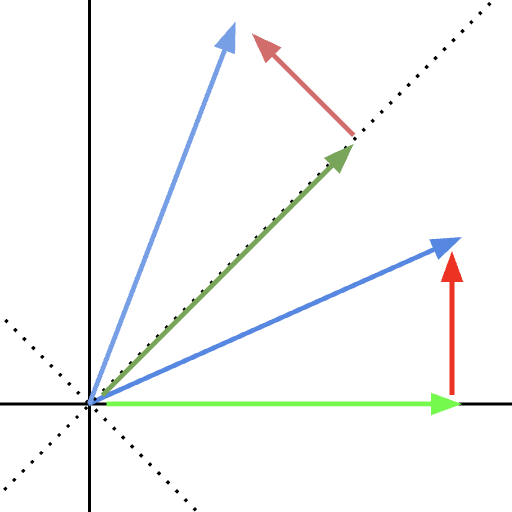
\includegraphics[scale=1]{rotation.png}
  \caption{A vector with coordinates in the standard basis,
    then rotated, has the same coordinates in the rotated
    basis since the basis vectors rotate with the vector.}
  \label{fig:rotation}
\end{figure}

\newpage

\section{Code}

The code is fairly simple; we start at the initial position and update
according to equation \eqref{eq:discrete}, arbitrarily taking a (relatively)
small step size of \( 10^{-3} \). This yields the same curve as if we
multiplied by \( \norm{\vec{r}} \) or if we used the analytic form in equation
\eqref{eq:solution}. To determine when to stop the simulation, we can end
after a certain number of iterations or after convergence (when we are a
certain \( \varepsilon \) distance from \( \vec{0} \), which is equivalent
to checking \( \norm{\vec{r}} < \varepsilon \)). To numerically compute the
arc length, we assume our step size is small enough such that when moving to
the next point, we assume the curve is perfectly approximated by the line
between the next point and the current point, i.e. the direction hasn't changed
in between. We simply sum up the lengths of the adjacent pairwise steps \(
\norm{\vec{r}_{n + 1} - \vec{r}_n} \). Finally, we record each \( \vec{r}_i
\) and graph each point in Matplotlib to generate \autoref{fig:missile}.

\newpage

\begin{minted}[label=simulation code,fontsize=\footnotesize]{python}
from typing import Callable
import numpy as np
import matplotlib.pyplot as plt

P0 = np.array([1, 1])  # initial position
ALPHA = np.deg2rad(60) # angle
VEL = 1e-3             # velocity
MAX_ITERS = 10**5      # maximum number of iterations 
EPSILON = 1E-3         # distance until convergence

# rotation matrix
T = np.array([[np.cos(ALPHA), -np.sin(ALPHA)],
              [np.sin(ALPHA),  np.cos(ALPHA)]])

def update1(r: np.array) -> np.array:
    """ Updates the position with a normalized velocity. """
    return r + -VEL*T@(r/np.linalg.norm(r))

def update2(r: np.array) -> np.array:
    """ Updates the position with proportional velocity. """
    return r + -VEL*T@r

def curve(t: float) -> np.array:
    """ Analytical parametrization of the missile's path. """
    gamma = np.sin(ALPHA)
    x = P0[0]*np.array([np.cos(gamma*t), -np.sin(gamma*t)])
    y = P0[1]*np.array([np.sin(gamma*t),  np.cos(gamma*t)])
    return np.exp(-t*np.cos(ALPHA))*(x + y)

def simulate(update: Callable[[np.array], np.array],
             criterion: str="iterations", max_iters: int=MAX_ITERS) -> tuple:
    """ Simulates the missile's path by discrete sampling. """
    iters = lambda t, r: t < max_iters
    criteria = {
        "iterations": iters,
        "distance": lambda t, r: np.linalg.norm(r) > EPSILON and iters(t, r),
    }
    criterion = criteria.get(criterion, criteria["iterations"])

    points = [P0]
    arc_length = 0
    t = 0
    while criterion(t, points[-1]):
        points.append(update(points[-1]))
        arc_length += np.linalg.norm(points[-1] - points[-2])
        t += 1
    return tuple(zip(*points)), arc_length, t

def sample(curve: Callable[[float], np.array],
           start: float, stop: float, step: float) -> zip:
    """ Samples a parameterized curve along an interval. """
    return zip(*(curve(t) for t in np.arange(start, stop, step)))

if __name__ == '__main__':
    (x1, y1), _, iters = simulate(update1, "iterations", 10000)
    (x2, y2), arc_length, iters = simulate(update2, "distance")
    print(f"arc length/initial distance: {arc_length/np.linalg.norm(P0):.3f}")
    print(f"{' '*18}1/cos({np.rad2deg(ALPHA):.0f}): {1/np.cos(ALPHA):.3f}")

    fig, ax = plt.subplots()
    ax.set_aspect("equal")

    plt.plot(*((np.arange(0, 1, 0.01),)*2), "bo", label=r"$\alpha = 0$")
    # plt.plot(x1, y1, "bo", label="arc length")
    plt.plot(x2, y2, "go", label=r"simulated")
    plt.plot(*sample(curve, 0, 10, 0.1), "ro", label="analytical")

    plt.title(r"Missile Trajectory for $\alpha = \pi/6$")
    plt.xlabel("x")
    plt.ylabel("y")
    plt.legend()
    plt.tight_layout()
    plt.savefig("missile.png")
    # plt.show()

\end{minted}

% \printbibliography
\end{document}
